\documentclass[preprint]{revtex4-1}
\usepackage{graphicx}
\usepackage{epstopdf}
\usepackage{amsmath}
\usepackage{hyperref}
\usepackage{booktabs}
\usepackage{color}

\usepackage{SIunits}
\newcommand{\wstar}{-0.023}
\newcommand{\Qstar}{0.25}

\setlength{\tabcolsep}{10pt}

\newenvironment{sistema}%
  {\left\lbrace\begin{array}{@{}l@{}}}%
  {\end{array}\right.}


\begin{document}
\title{Roles of icosahedral order in hard spheres glass transition} 
%\title{Role of structural heterogeneity of the supercooled liquid\\ in the crystallization of hard spheres}
%\title{On the origin of polymorphism during the nucleation of hard spheres}
%\title{On the origin of crystal polymorphism in hard spheres}
%\title{Selection principle of polymorphs upon crystallization \\ in hard spheres}
%\title{Role of orientational order in the crystallization of hard spheres}
%\title{On the microscopic mechanism of crystallization in hard spheres:\\ role of bond
%orientational ordering}
%\title{Crystal Polymorphism starts before crystallization}
%\title{Crystal Polymorphism starts before crystallization}
%\title{Crystal Polymorphism before crystallization}


\author{Mathieu Leocmach} 

\author{Hajime Tanaka}
\affiliation{ {Institute of Industrial Science, University of Tokyo, 4-6-1 Komaba, Meguro-ku, Tokyo 153-8505, Japan} }

\date{Received \today}

\begin{abstract}
\textbf{
A link between local structural ordering and slow dynamics has recently attracted much attention from the context of the origin of glassy slow dynamics~\citep{cavagna2009supercooled,BerthierR}. There have been a few candidates for such structural order, icosahedral order~\cite{steinhardt1983boo,tarjus2005fba}, exotic amorphous order~\cite{lubchenko2007}, and crystal-like order~\cite{tanaka2010critical}. Each type of order is linked to a different scenario of glass transition. Thus, revealing the order responsible for slow dynamics is crucial for our understanding of glass transition. Here we experimentally access local structural order in polydisperse hard spheres by its particle-level observation with confocal microscopy. We identify the key structures as icosahedral and \textmd{\textsc{fcc}}-like order, excluding any other simple local symmetry. We find that both types of order are statistically associated with slow particles. However, when approaching the glass transition, the icosahedral order do not grow in size whereas crystal-like structures grow. It is the latter that governs the dynamics and is linked to dynamic heterogeneity. This questions the direct roles of the icosahedral ordering in glassy slow dynamics and stresses the importance of the structural order compatible with the avoided first order transition, crystallization. Our finding also suggests that the growing lengthscale of structural order is essential for the slowing down of dynamics and the nonlocal cooperativity in particle motion. 
}
\end{abstract}
\maketitle



%The possibility of a non-crystalline order has been discussed mainly in relation to the long standing problem of the glass transition. Even %so, its role remains unclear: actively slowing down the system or avoiding crystal formation. This issue may be crucial in the design of good %glass formers.

Upon cooling, a liquid usually undergoes a first order transition to an ordered ground state (crystal or quasi-crystal). However, it is generally possible to avoid the transition and to form a metastable supercooled liquid. Upon further cooling the dynamics slows down dramatically by many orders of magnitude, leading to the impossibility to equilibrate the system in the experimental time scale below a temperature $T_g$ named the glass transition temperature. The nature of the glass transition (thermodynamic or kinetic, structural or purely dynamical) is still matter of debates after decades of intensive research (see~\citep{cavagna2009supercooled,BerthierR} for comprehensive reviews).

A part of the answer is believed to come from the dynamics in itself: a supercooled liquid is dynamically heterogeneous (see~\citep{BerthierR} for a review) and the characteristic size of the dynamical heterogeneity is growing when approaching the glass transition~\citep{yamamoto1998, Donati1999a}. The dynamical arrest may then be the analogue of the slowing down observed near a critical point when the characteristic size of the fluctuations diverges, although slowing down at a particle level is absent in ordinary critical phenomena. Here we note that the length scale defined by the dynamical heterogeneity is not static (one-time spatial correlation) but dynamic (two-time spatial correlation). 

In order to unveil static quantities, it is tempting to link dynamical heterogeneity to structural heterogeneity. Stable structures should move less than unstable ones.~\citet{Widmer-Cooper2005} demonstrated that the initial configuration of a simulation, independently of the initial dynamics, has a role in the heterogeneity of the dynamics. \citet{Berthier2007} pointed out later that this influence does not exist at the particle level, but on larger scales: medium-range particle configuration can be statistically linked to medium range dynamical heterogeneity. However these arguments are based on the iso-configurational ensemble (starting again and again simulations with different dynamics but with the same initial configuration), a method that has no experimental equivalent yet.

Given that a glass shows no long-range periodic order, structures different from a crystal, icosahedral  ~\cite{steinhardt1983boo,tarjus2005fba} or amorphous order \cite{lubchenko2007}, are most often pointed as responsible for the dynamical arrest. Since the pioneering work of Frank, icosahedral order is the archetypal model of amorphous structures~\citep{Spaepen2000}. Locally, an icosahedron maximises the density of packing, but its five-fold symmetry is incompatible with long-range periodicity. Geometrical frustration associated with icosahedral ordering is proposed to be crucial for vitrification ~\cite{steinhardt1983boo,tarjus2005fba}. It was also proposed that the percolation of icosahedral order is responsible for glass transition~\cite{Tomida1995}.  Evidence of icosahedral ordering has indeed been found in very dense hard sphere packings~\citep{Bernal1960, Clarke1993, Malshe2011}, in various simulation models~\citep{steinhardt1983boo, Tomida1995, Doye2003, Pedersen2010, Coslovich2011} and more recently in experimental dense metallic liquids~\citep{Reichert2000, Celino2007} and glasses~\citep{Luo2004, Wang2011}.

Icosahedral order (or more generally locally favoured structures of the liquid) plays a central role in the spin-glass-type theory~\cite{steinhardt1983boo} and the frustration-limited domain theory of the glass transition (see~\citep{tarjus2005fba} for a review). The former theory consider the icosahedral ordering under frustration. On the other hand, the latter theory takes as a reference state an unfrustrated icosahedral order existing in a curved space, even if and because this reference state is impossible to reach for the real system. If the space were curved, the locally preferred order of the liquid (icosahedral) would form a continuous ordered phase upon cooling. In the  euclidean space, however, this transition is avoided, yet the avoided transition temperature still acts as a critical point giving rise to diverging lengthscales (icosahedral domain size and defect size) that would explain the dynamical arrest. This theory suggests that the frustration-limited domains are the origin of the dynamical heterogeneity. Yet, to our knowledge, numerical systems where a link between icosahedral order and dynamical heterogeneity has been observed~\citep{Doye2003, Pedersen2010, Coslovich2011}, have a (quasi)crystalline ground state including icosahedra. Thus, icosahedra should be regarded as a structural motif linked to the crystalline ground state in these systems. These results, thus, do not support the spin-glass or frustration-limited domain approaches, but rather the crystal-based approach (see below).  

An other way of explaining the phenomenology of the glass transition is based on the structure of the crystal. The crystallisation, even if avoided, may have an influence on the supercooled fluid or the glass~\citep{TanakaGJPCM, Cavagna2003} and is taken as reference state. Simulations~\cite{tanaka2010critical, Pedersen2010, Coslovich2011} and experiments~\citep{tanaka2010critical} show that a local order compatible with the ground state (crystal) symmetry does extend on medium range in several model supercooled systems. These transient but relatively stable structures seem to be correlated with the slow regions because they are low free-energy configurations. Furthermore, they lack extended positional order and thus could not be detected by macroscopic diffraction experiments.

In the present work, we focus on the colloidal (hard spheres) supercooled liquid \cite{pusey1987ogt} for two reasons. First, hard sphere-like colloidal particles can be tracked by confocal microscopy, giving access to the positions and dynamics of individual particles \cite{kegel2000swe, weeks2000}, thus allowing microscopic analysis of the dynamical and structural heterogeneity. Second, hard spheres have a well defined crystalline ground state of face-centred-cubic (\textsc{fcc}) or hexagonal-close-packed (\textsc{hcp}) symmetry and locally favoured structures of icosahedral symmetry. This allows us to distinguish the different scenarios of glass transition, in particular, the frustration-limited domain scenario and the medium range crystalline order scenario.



We were able to follow the volume fraction dependence of the dynamics over nearly three orders of magnitude (see Fig.~\ref{fig:vft}), confirming the basic phenomenology observed in experiments~\citep{pusey1987ogt, kegel2000swe, weeks2000, BerthierR} as well as simulations~\citep{tanaka2010critical} of similar systems: super-Arrhenius dependence of the relaxation time $\tau_\alpha$ upon $\phi$, that we fit by the Vogel-Fulcher-Tammann law, 
$\tau_\alpha=\tau_\alpha^0 \exp(D\phi/(\phi_0-\phi))$ ($D$: the fragility index), non-Gaussianity of the dynamics peaking at $t^{dh}(\phi)$, and dynamical heterogeneity of growing size $\xi_u$. 



The local structures of our suspensions are identified by a detailed analysis of Steinhardt's bond orientational order (\textsc{boo})~\citep{steinhardt1983boo}, including original improvements (see Methods). Figure~\ref{fig:maps} summarizes our structure identification results. We find the distinctive signature of medium ranged crystalline order (\textsc{mrco}) of \textsc{fcc} type, without excluding some \textsc{hcp}. We stress that \textsc{mrco} does not correspond to crystal nucleus and accompanies little increase in the local density. We find no trace of \textsc{bcc}-like structure. As for the aperiodic structures, icosahedral order stands out without any other obvious rivals (Dodecahedron are present but can be considered as twisted icosahedron).



We establish that in our system the tendency towards icosahedral order is best monitored by $w_6$, whereas $Q_6$ is the natural crystal-like order parameter (see Methods for the definitions of $w_6$ and $Q_6$). The population of local structures in the $(w_6,Q_6)$-plane is shown in Fig.~\ref{fig:maps}\textbf{c-d}, which confirms that the two tendencies are present in the supercooled liquid of hard spheres. In particular, to our surprise, icosahedra are present even at a relatively low volume fraction (Fig.~\ref{fig:maps}\textbf{d}). Both tendencies become more pronounced with deeper supercooling (Fig.~\ref{fig:maps}\textbf{c}). Furthermore, Fig.~\ref{fig:maps}\textbf{c} show clearly that icosahedral order and crystalline order are incompatible and frustrate one another.



In the introduction we mentioned the dynamic propensity invented by~\citet{Widmer-Cooper2005} as a trick only accessible via simulations. In our system, since we know the relevant structural order parameters ($w_6$ and $Q_6$), we can compute the square displacement of all the particles with the same initial local structure (iso-bond order ensemble). We define the $w_6$-propensity as
\begin{equation}
	\mathcal{P}r(w_6, t) \equiv \left\langle \frac{
		\sum\limits_i{
			\left\|\vec{r_i}(t)-\vec{r_i}(0)\right\|^2 \delta(w_6^i-w_6)
			}
	}{
		\sum\limits_i{\delta(w_6^i-w_6)}
	}\right\rangle 
	\label{eq:bo_propensity}
\end{equation}
where the brackets denote ensemble averaging. $\mathcal{P}r(Q_6, t)$ and $\mathcal{P}r(w_6, Q_6, t)$ can be defined in the same way. Note that this \emph{bond order dynamic propensity} is accessible even in a system that cannot be restarted \emph{ab libitum} from exactly the same overall configuration.

Figure~\ref{fig:msd_Q6_w6} shows the bond order propensity (calculated at $t^{dh}$). Both structural order parameters have a clear correlation with the dynamics: the more structured is the environment, the more likely the particle will be slow. For all volume fractions, the propensity displays the same linear dependence upon $w_6$ (Fig.~\ref{fig:msd_Q6_w6}\textbf{b}). Once scaled by the mean square displacement all points collapse on the same line. This is not the case for the $Q_6$ dependence (Fig.~\ref{fig:msd_Q6_w6}\textbf{c}) which is more and more pronounced with increasing the degree of supercooling. In our most deeply supercooled sample, the crystal-like environments can be in average ten times slower than the bulk; whereas even the almost perfect icosahedra are in average only $40\%$ slower than the bulk. Our results also show that slow dynamics is not due to exotic amorphous order, which should have low $Q_6$, at least in our system. 

To explain our propensity data, we can refer to the cage picture, where a particle is considered as trapped in the cage formed by its neighbours. Once the particle has escaped from its cage, it is free to diffuse. In general, this picture is not correct due to dynamical heterogeneity, or nonlocal cooperativity of motion. However in the case of the icosahedral environment it seems to hold: the normalisation by the bulk \textsc{msd} takes into account the diffusion once out of the cage, and the remaining universal dependence upon $w_6$ holds the information about the ``quality'' of the cage. Efficient packing makes the 13 particles icosahedra more stable than a disordered structure. Thus the central particle has a low probability to escape from its cage and start diffusing. After that it diffuses in average like any other particles. This suggests that the influence of icosahedral order on the dynamics is only local because of its isolated character. By contrast the non-trivial $\phi$ dependence of the $Q_6$-propensity calls for nonlocal explanations.

To observe the ordered regions in real space, we define the thresholds $w_6^*$ and $Q_6^*$ so that the bond order propensity at the threshold is half between the bulk and the (extrapolated) prefect structure. In our most deeply supercooled sample, this criterion yields $w_6^* = \wstar$ and $Q_6^* = \Qstar$. These thresholds are arbitrary but coherent with each another. We display in Fig.~\ref{fig:3D}\textbf{c} typical configurations of the ordered neighbourhoods in our deepest supercooled sample. With our thresholds, we see only small patches of icosahedral order that are not reaching medium range; whereas clusters of crystal-like order are much larger than icosahedral clusters and their sizes reach medium range. 



Consistently, we were not able to extract a lengthscale associated with the sole icosahedral order that would grow when approaching the glass transition. By contrast, the spatial extent of crystal-like order is well described by $G_6(r)$, the spatial correlation function of $Q_{6 m}$ (see, e.g., cite{tanaka2010critical}). Both dynamical and structural lengthscales are increasing while approaching the glass transition in a coherent manner (the inset of Fig.~\ref{fig:vft}). We can see that the growth of both dynamic and static correlation length can be well expressed by the power law,   $\xi_{u,6} \propto (\phi/(\phi_0-\phi))^{-\nu}$ with $\nu=2/3$. In agreement with~\citep{tanaka2010critical} it suggests that the dynamical heterogeneity in hard spheres is a manifestation of critical-like fluctuations of the crystal-like bond orientational order parameter, and not those of icosahedral or amorphous order. In relation to this, we stress that $G_6(r)$ is constructed from the coarse-grained \textsc{boo} and thus not sensible to aperiodic structures such as icosahedral or amorphous order. 

Of course, one can set a more permissive threshold on $w_6$ and observe more icosahedra. A percolating network of icosahedral neighbourhood can even be found at a high volume fraction if the threshold encompasses enough particles. However, the imperfect icosahedra particles that must be included to form this network have a mobility comparable to the bulk (Fig.~\ref{fig:msd_Q6_w6}\textbf{b}). Furthermore, we checked that this percolation is of the 3D random percolation class (cluster size distribution follows a power-law of exponent $\approx 2.1$), meaning that a comparable network could be obtained by picking randomly the same number of particles. We conclude that the concept of icosahedral network is not physically meaningful at least in our system.

As a final but an intuitive check, we were able to compare the spatial repartition of crystal-like order (Fig.~\ref{fig:3D}\textbf{d}) and slow particles (Fig.~\ref{fig:3D}\textbf{e}). As shown in~\citep{Berthier2007}, the correlation between structure and dynamics is not a one-to-one correspondence at the particle level but a statistical relationship on larger length scales. We were able to show visually this correlation by calculating the square displacement of each particle over $2\tau_\alpha\approx 4.5t^{dh}$ which allow to accumulate many rearrangement events; and by coarse-graining this value over the particle's neighbours~\citep{Berthier2007} (see Eq.~\ref{eq:Mu}). Fig.~\ref{fig:3D}\textbf{e} displays the $10\%$ slowest particles according to this criterion and their neighbours. The correlation of shape and size is visible between Fig.~\ref{fig:3D}\textbf{d} and Fig.~\ref{fig:3D}\textbf{e}, however no such correlation can be found between icosahedral particles (Fig.~\ref{fig:3D}\textbf{c}) and slow regions.



We have demonstrated that supercooled hard-sphere liquids display local icosahedral ordering while having structural ordering linked to the avoided crystalline (\textsc{fcc}) ground state. Both types of packing are efficient and thus locally favoured. Yet the icosahedral order remains local even at deep supercooling and (consistently with the arguments of~\citep{Berthier2007}) is not able to influence significantly the global dynamics. By contrast, the slowing down associated with the crystal-like symmetry is long-lived, nonlocal and the characteristic length scale of the crystalline order grows when approaching the glass transition in the same way as the dynamical heterogeneity. This suggests that the structural origin of the dynamical arrest is linked to the avoided crystallisation and not to the condensation of the local (icosahedral) order of the liquid. We note that the development of structural order and its link to dynamic heterogeneity are at odds with purely kinetic scenarios of glass transition. 

For some systems, the first order transition avoided upon supercooling leads to a symmetry compatible with icosahedral order. The symmetry-breaking phase can be a quasi-crystal~\citep{Doye2003} or a Frank-Kasper crystal like recently demonstrated for Wahnstr\"om mixture~\citep{Pedersen2010}. In that case, the amorphous order cannot be distinguished from the defective crystalline order that slows down the system, so the amorphous order seems to play a role in the slowing down. However, we showed here that when the amorphous order is not compatible with the crystal symmetry, its role in the slowing down seems to be minor.

We do not say that the local order of the liquid (icosahedral) is unimportant in the glass transition. Actually it plays a role in preventing the first order transition (crystallisation) to append, thus allowing supercooling and the glass transition \cite{TanakaMJPCM}. Furthermore, this frustration against crystallisation may be linked to the fragility of the glass former~\citep{TanakaGJPCM,tanaka2010critical}. Competing crystal-like and non-crystal-like orderings may be important in many glass-forming systems covering colloidal, molecular, polymeric, oxide, chalcogenide, and metallic glasses. In particular, our finding may have important implications on the physical mechanism responsible for the high glass-forming ability of bulk metallic glassformers~\cite{Wang2004}. 

\vspace{1cm}
\noindent
\textbf{Methods}

We used \textsc{pmma} (poly(methyl methacrylate)) colloids sterically stabilized with methacryloxypropyl terminated \textsc{pdms}(poly(dimethyl siloxane)) and fluorescently labelled with rhodamine isothiocyanate chemically bonded to the \textsc{pmma}. The size distribution, as characterised by scanning electron microscopy imaging, showed a long tail toward small sizes, leading to about $6\%$ polydispersity. This amount of polydispersity allows us to avoid crystallisation but is too low for fractionation to append~\citep{Fasolo2003}. The colloids were suspended in a solvent mixture of cis-decalin and cyclohexyl-bromide for both optical index and density matching. To screen any (weak) electrostatic interactions, we dissolved tetrabutylammonium bromide salt, to a concentration of \unit{300}{\nano\mole\per\liter}~\citep{royall2005}. The estimated Debye screening length is \unit{100}{\nano\metre}, well below the length scale of the colloids. To avoid errors due to the swelling of the particles, their size was measured in the same solvent by the following technique: short-ranged depletion attraction was induced by adding non-adsorbing polystyrene to a dilute suspension to drive particles into contact; the position of the first peak of the $g(r)$ gave the diameter $\sigma = \unit{3.356\pm0.03}{\micro\meter}$.

After careful shear melting, the samples are filled into square $\unit{500}{\micro\metre}$ capillaries (Vitrocom). The most deeply supercooled sample showed a slight indication of sedimentation even after careful density matching. To avoid this effect we used a thinner $\unit{100}{\micro\metre}\times\unit{1}{\milli\metre}$ cell. The data was collected on a Leica SP5 confocal microscope, using \unit{532}{\nano\meter} laser excitation. The temperature was controlled on both stage and objective lens, allowing a more precise density matching. Our polydisperse colloids were detected using a novel multi-scale algorithm that will be described elsewhere, allowing us to retrieve both position and size of each particle with about $1\%$ precision. The large size of our colloids allows a comparable precision in position for both in-plane and out-of-plane coordinates. The particles are tracked in time to extract dynamical informations. Typically $\approx 5000$ trajectories can be followed over a few structural relaxation times.



\citet{steinhardt1983boo} defined the \textsc{boo} of the $\ell$-fold symmetry as a $2\ell+1$ vector:
\begin{equation}
	q_{\ell m}(i) = \frac{1}{N_i}\sum_{0}^{N_i} Y_{\ell m}(\theta(\vec r_{ij}),\phi(\vec r_{ij}))
	\label{eq:qlm}
\end{equation}
where the $Y_{\ell m}$ are spherical harmonics. In the analysis, one uses the spherical invariants defined as:
\begin{align}
	q_\ell =& \sqrt{\frac{4\pi}{2l+1} \sum_{m=-\ell}^{\ell} |q_{\ell m}|^2 }\label{eq:ql}\\
	w_\ell =& \sum_{m_1+m_2+m_3=0} 
			\left( \begin{array}{ccc}
				\ell & \ell & \ell \\
				m_1 & m_2 & m_3 
			\end{array} \right)
			q_{\ell m_1} q_{\ell m_2} q_{\ell m_3} \label{eq:wl}\\
	\hat{w}_\ell =& w_\ell{\left( \sum_{m=-\ell}^{\ell} |q_{\ell m}|^2 \right)}^{-\frac{3}{2}}
\end{align}
where the term in brackets is the Wigner 3-j symbol. Note that the popular~\citep{steinhardt1983boo,Lechner2008} $\hat{w}_\ell$ can show a large norm if its denominator (or $q_\ell$) has small values (particle with low $\ell$-fold symmetry). Therefore, we have used here mostly the unreduced $w_\ell$ that pulls clearly apart highly symmetric particles from the fluid distribution.

Following~\citet{Lechner2008}, one can coarse-grain the tensorial \textsc{boo} over the neighbours:
\begin{equation}
	Q_{\ell m}(i) = \frac{1}{N(i)+1}\left( q_{\ell m}(i) +  \sum_{j=0}^{N(i)} q_{\ell m}(j)\right) 
	\label{eq:Qlm}
\end{equation}
and define coarse-grained invariants $Q_\ell$ and $W_\ell$ in the same way as Eqs.~(\ref{eq:ql}) and (\ref{eq:wl}). Structures with some amount of periodicity (crystalline) are then much easier to tell apart~\citep{Lechner2008}. However, non-periodic structures like icosahedra see their $Q_\ell$ and $W_\ell$ buried into the liquid distribution. With this in mind, we looked for periodic structures in the $\lbrace Q_\ell, W_\ell\rbrace$ space, and for aperiodic structures in the $\lbrace q_\ell, w_\ell\rbrace$ space, with $\ell=4,6,8,10$.

In both Eqs.~(\ref{eq:qlm}) and (\ref{eq:Qlm}), the sum runs over the ``neighbours'' of particle $i$. The definition of the neighbours is crucial for the consistency of the analysis. The most popular criterion in literature is that particles closer than $R_{max}$ are neighbours, with $R_{max}$ often fixed at the first minimum of $g(r)$. However, we find that this criterion has two major drawbacks: no account of polydispersity and negative correlation between the number of neighbours and the value of the $q_\ell$ (this effect is less pronounced after coarse-graining). To account for the polydispersity, we used a threshold in the scaled distance $\hat{r}_{i j} = r_{i j} /(\sigma_i+\sigma_j) < \hat{R}_{max}$, with $\hat{R}_{max}$ corresponding to the first minimum of $g(\hat{r})$. This allows us to look for structures without assumptions on the number of neighbours. 

We made a first round of analysis using this threshold definition, constructing maps similar to Fig.~\ref{fig:maps} but nosier. These maps allowed us to discard the possibility of \textsc{bcc} (high $Q_6$, low $Q_4$, high $Q_{10}$) and generally any structure except \textsc{fcc} (high $Q_6$, high $Q_4$ and $W_4<0$), \textsc{hcp} (high $Q_6$ and $W_4>0$) or icosahedron (very negative $w_6$, high $q_6$ and $q_{10}$). Dodecahedron can be found for $w_6>w_6^{dod}\approx -0.00782$, \emph{i.e.}, between the liquid and the icosahedral order. We are thus left with structures where the particles naturally have 12 neighbours. We then took a new \textsc{boo} analysis, this time taking the first 12 closest particles (in $\hat{r}$) as neighbours. This criterion reduces the noise in the distribution of the invariants and makes detected structures more easily comparable with crystallographic archetypes. It also avoids artefacts near $R_{max}$ in the correlation functions. The figures presented here were constructed from this second round of analysis.

This second definition of the neighbours is used consistently in the coarse graining of the square displacements:
\begin{equation}
	\bar{\mu}_i(t) = \frac{1}{N(i)+1}\left( \mu_i(t) + \sum_{j=0}^{N(i)} \mu_j(t) \right) 
	\label{eq:Mu}
\end{equation}
where $\mu_i(t) = \left\|\vec{r_i}(t)-\vec{r_i}(0)\right\|^2$ and the neighbours are defined at initial time. Note that we recover the correlation between crystalline order and slowness by two independent methods: directly in the instantaneous \textsc{boo} space via the propensity on moderate times; and indirectly via the positions and shapes of the (short time averaged) ordered regions coherent with those of the slowest regions (on long times). In the former method, the quality of the statistics comes from ensemble averaging over the many realisations of each structure. In the later method, it comes from both coarse graining and the length of the trajectories that allow to accumulate many rearrangement events.

%\bibliographystyle{apsrev4-1}
\bibliographystyle{naturemag3}
\bibliography{ico_dyn}

\vspace{2cm}
\noindent
\textbf{Acknowledgments}

\noindent
The authors thank Paddy Royall and John Russo for fruitful discussions. 
This work was partially supported by a grant-in-aid from the 
Ministry of Education, Culture, Sports, Science and Technology, Japan. 

\clearpage

\begin{figure}
\begin{center}
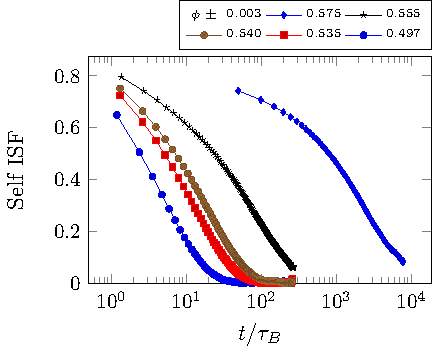
\includegraphics{generate_figures-figure0.pdf}
\end{center}
\caption{\textbf{Dynamics of the system.} {\bf a,} Decay of the self-intermediate scattering function computed from the positions for several volume fractions. {\bf b,} The structural relaxation time $\tau_\alpha$ and the characteristic time of the dynamic heterogeneity $t^{dh}$ scaled by the Brownian time $\tau_B$ as a function of $\phi$. The solid curve is the VFT fit of $\tau_\alpha$. Inset: Dynamical ($\xi_u$) and structural correlation length ($\xi_6$). Solid curves are power-law fits (see text).}
	\label{fig:vft}
\end{figure}

\clearpage

\begin{figure}
\begin{center}
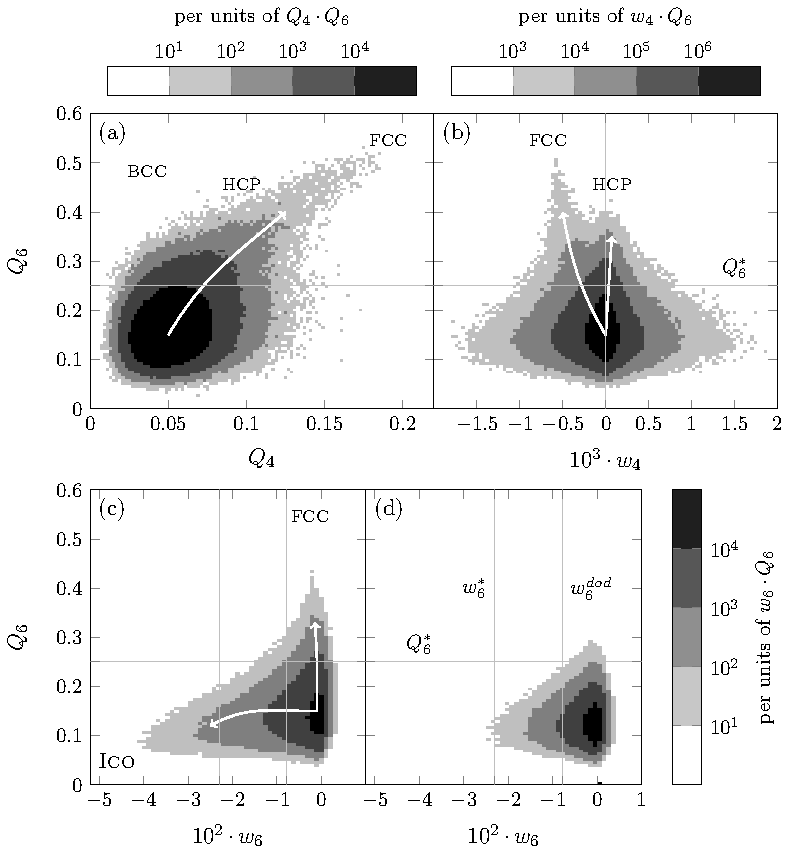
\includegraphics{generate_figures-figure1.pdf}
\end{center}
\caption{\textbf{Population of local structures function of the }\textsc{boo}\textbf{ parameters}. The values of \textsc{boo} parameters for a perfect structure are indicated by its name's position on each map. {\bf a-c,} For our deepest supercooled sample ($\phi=0.575\pm 0.03$) in the $(Q_4,Q_6)$-plane ({\bf a}), $(w_4,Q_6)$-plane ({\bf b}) and $(w_6,Q_6)$-plane ({\bf c}). {\bf d,} The same as {\bf c} but for a liquid near the freezing point ($\phi = 0.497 \pm 0.03$). Colour represents the probability to find the structure (log scale). The arrows stress the ordering tendencies: the tendency towards \textsc{fcc} is always visible, a weak tendency towards \textsc{hcp} can also be distinguished in {\bf b}, and the tendency towards icosahedral order is visible in {\bf c}.}
	\label{fig:maps}
\end{figure}

\clearpage

\begin{figure}
\begin{center}
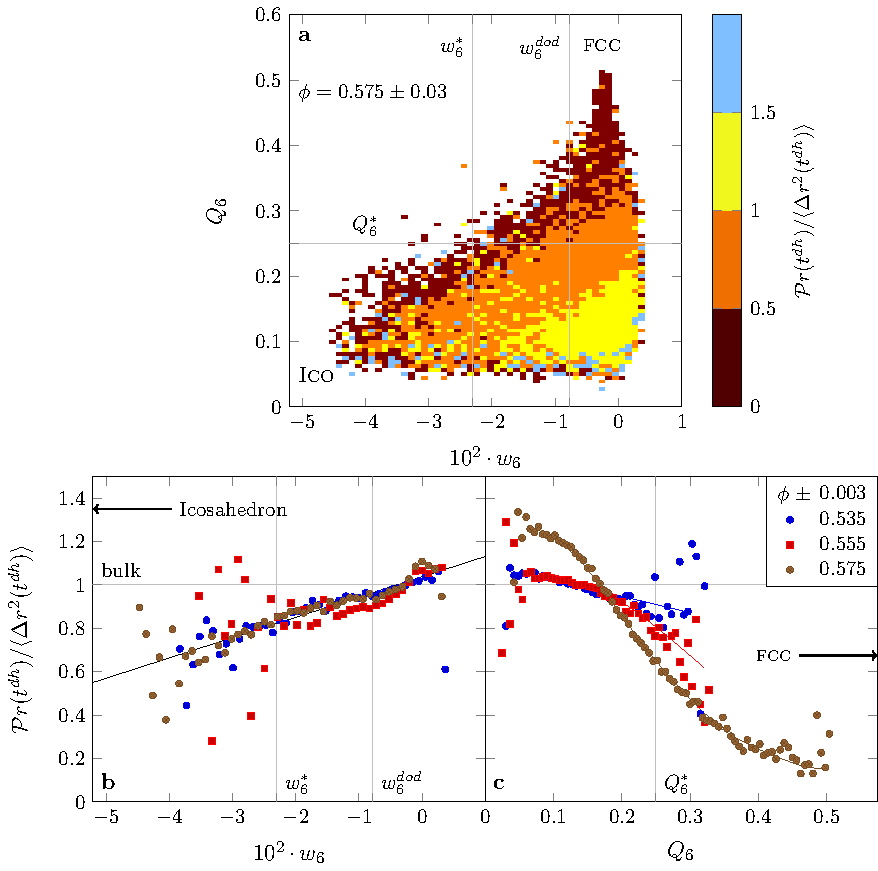
\includegraphics{generate_figures-figure2.pdf}
\end{center}
\caption{\textbf{Bond order propensity.} {\bf a,} Normalised propensity in the $(w_6, Q_6)$-plane for our most deeply supercooled sample. The colour scale is saturated at $1.5$ times the bulk mean square displacement. {\bf b-c,} Normalised propensity for icosahedral and crystalline order parameters respectively. Bulk mean square displacement is scaled to be at 1. Perfect structures are on the edge of each plot. The lines are a guide for the eye, stressing the collapse of the $w_6$-propensity at all volume fractions in {\bf b} and the absence of collapse in {\bf c}. The scattering at low volume fractions is due to poor averaging of rare structures.}
	\label{fig:msd_Q6_w6}
\end{figure}

\clearpage

\begin{figure}
\begin{center}
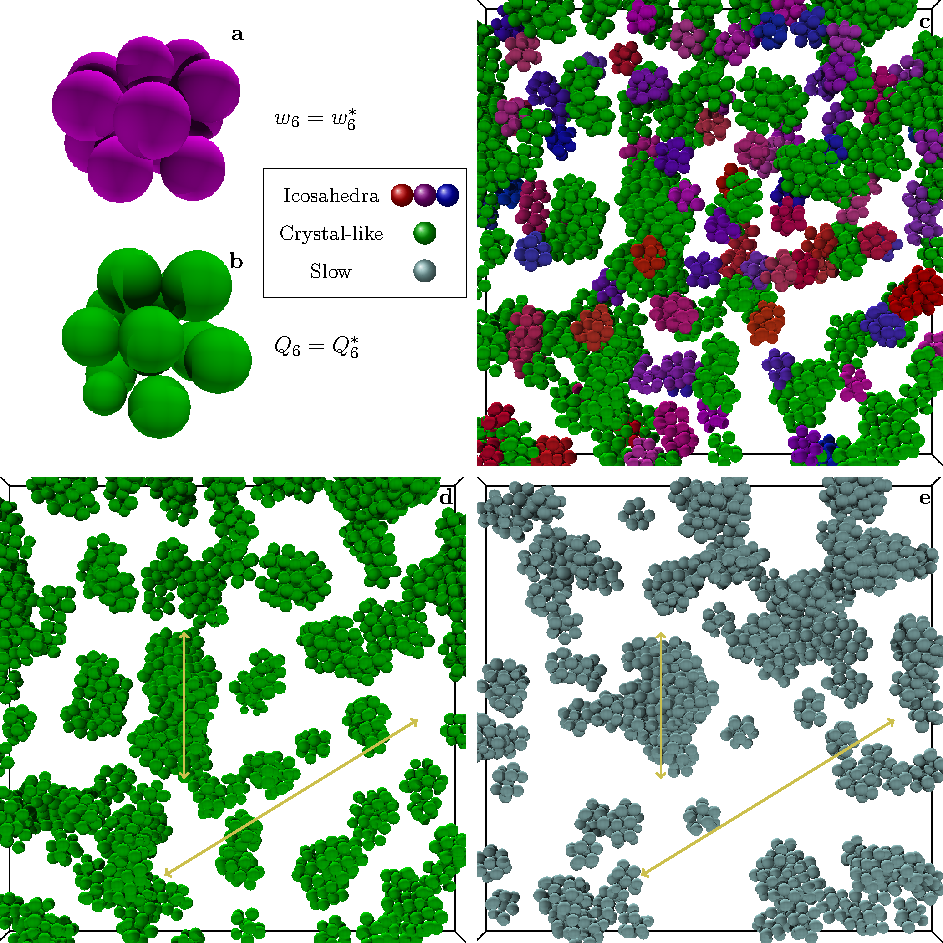
\includegraphics{generate_figures-figure3.pdf}
\end{center}
\caption{\textbf{Computer reconstruction from confocal microscopy coordinates of a typical configuration in our most deeply supercooled sample.} Depth is $\sim 12\sigma$. Only particles of interest and their neighbours are displayed. Each particle is plotted with its real radius.  Example of \textbf{a} distorted icosahedron and \textbf{b} crystal-like cluster at the respective threshold values. \textbf{c,} Bond ordered particles. Two icosahedral particle are shown in the same shade if they belong to the same cluster. If a particle is neighbouring both kind of structures, it is displayed as icosahedral. \textbf{d,} Crystal-like particles alone (the order parameter was averaged over $t^{dh}/2$). \textbf{e,} Slow particles (see text). The arrows stress the correlation between \textbf{d} and \textbf{e}. Due to particles going in and out of the field of view, the edges of \textbf{d} and \textbf{e} where not accurate and have been removed.}
	\label{fig:3D}
\end{figure}

\end{document}